\documentclass{article} % For LaTeX2e
\usepackage{nips15submit_e,times}
\usepackage{hyperref}
\usepackage{url}
\usepackage{caption}
\usepackage{refstyle}
\usepackage{amsmath}
\usepackage{times}
\usepackage{epsfig}
\usepackage{graphicx}
\usepackage{amsmath}
\usepackage{amssymb}
\usepackage{algpseudocode}
\usepackage{algorithm}
%\usepackage{subcaption}
\usepackage{subfig}
\usepackage{listings}
\usepackage{tabu}
\usepackage{float}
\restylefloat{table}
%\documentstyle[nips14submit_09,times,art10]{article} % For LaTeX 2.09

\title{CSE 253 PA3. Deep Convolutional Network for Image Classification and Transfer Learning}


\author{
Siwei Guo \\
Department of Electrical and\\ 
Computer Engineering\\
University of California San Diego\\
San Diego, CA 92037 \\
\texttt{s9guo@eng.ucsd.edu} \\
\And
Jingyi Yang \\
Department of Electrical and\\ 
Computer Engineering\\
University of California San Diego\\
San Diego, CA 92037 \\
\texttt{jiy349@eng.ucsd.edu} \\
\And
XXX \\
Department of Electrical and\\ 
Computer Engineering\\
University of California San Diego\\
San Diego, CA 92037 \\
\texttt{xxx@eng.ucsd.edu} \\
\And
XXX \\
Department of Electrical and\\ 
Computer Engineering\\
University of California San Diego\\
San Diego, CA 92037 \\
\texttt{xxx@eng.ucsd.edu} \\
}

% The \author macro works with any number of authors. There are two commands
% used to separate the names and addresses of multiple authors: \And and \AND.
%
% Using \And between authors leaves it to \LaTeX{} to determine where to break
% the lines. Using \AND forces a linebreak at that point. So, if \LaTeX{}
% puts 3 of 4 authors names on the first line, and the last on the second
% line, try using \AND instead of \And before the third author name.

\newcommand{\fix}{\marginpar{FIX}}
\newcommand{\new}{\marginpar{NEW}}

\nipsfinalcopy % Uncomment for camera-ready version

\begin{document}


\maketitle

\begin{abstract}
Convolutional Neural Networks have been applied to visual tasks since the late 1980s, but were not popular until the mid-2000s when developments in computing power and the advent of large amounts of labeled data contributed to advancement. By comparing different models of CNN, AlexNet, GoogLeNet and a self-built one, GoogLeNet reports to have the highest accuracy of 99.2\%, AlexNet 98.5\%, and the self-build one 97.4\%.
\IfFileExists{contrib}{\input{contrib}}{.}
\end{abstract}

\section{Introduction}
Deep learning models have achieved remarkable results in image classification problems. This approach is more efficient and give much better result compare to traditional modelling approach. However, the learning process of Neural Network is not comprehensible compare to traditional method. Therefore, in this work, we trained three different CNN models on CIFAR-10 Dataset. First, we build a simple 6 layer shallow neural network. Then, we tried some other existing sucessful network models, AlexNet and GoogLeNet. We experiented different parameters, such as kernel size, different layers and other techniques.

\IfFileExists{contrib}{\input{contrib}}{.}

\section{Deep CNN for Image Classification}
Using images from CIFAR-10 Dataset, we used three architectures to test a CNN's accuracy vs the number of 
epochs. Specifically, we built an AlexNet with , partial GoogLeNet with 18 convolutions, and a self-built 
net with . Generally, the comparision between AlexNet and self-build network indicates how the depth of 
network influence the performance. The comparision between AlexNet and GoogLeNet shows how difference architecture
perform differently and Inception model's ability to speed up training process. We also tried different
parameters on self-build model to test maxpooling, kernel size, Xavier initialization and batch normalization. 



\subsection{AlexNet Model}
The first model we built was an AlexNet model. AlexNet has been proved to be a break through in the
field of deep learning and can achieve good performance. Follow the rule of "don't be a hero", we
first borrowed Alex Krizhevsky's model. We built an AlexNet with 5 convolutions and 3 fully connected
 layers and the diagram is show in \figref{alex} (right). The kernel size for each convolution 
 is 5, 5, 3, 3, 3 with batch normalization, Xavier initialization and Adam Optimizer. The accuracy 
 plot is also shown in \figref{alex} (left). For AlexNet, we reduced the size of convolution kernel 
 from 11x11 to 5x5 since our image size is relatively small. 11x11 kernel will take over 1/3 of the 
 image pixel and return a more global features instead of local features that we want. It also turns 
 out that 5x5 works better compare to 11x11 kernel in terms of both training speed and accuracy.

\begin{figure}[h]
    \centering
    \subfloat[Accuracy vs. Epoch]{{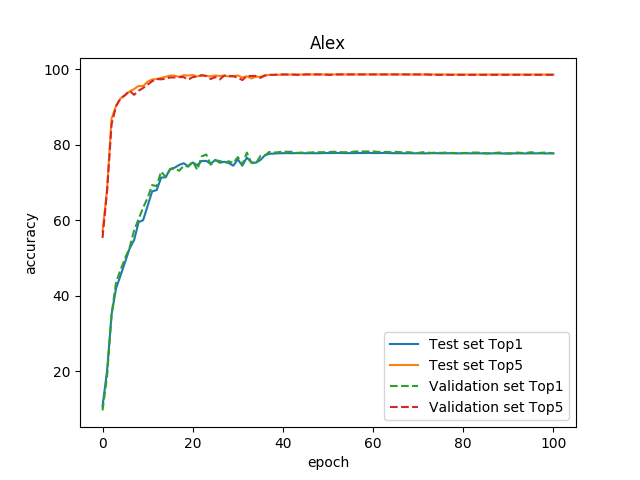
\includegraphics[width=6cm]{alexnet.png} }}
    \qquad
    \subfloat[Alex Net Diagram]{{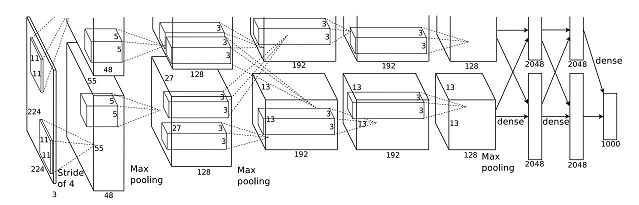
\includegraphics[width=6cm]{alexdiag.png} }}
    \caption{AlexNet Model}
    \label{fig:alex}
\end{figure}
 
 \subsection{Self-built Model}
 We also tried building a self-built architecture with 3 convolutions and 3 fully connected layers, 
 with kernel size 3, 3, 3. We added max pooling into self-build architecture since max pooling can 
 downsize the feature map and introduce some amount of translation invariance to the network. 
 Then we also add batch normalization after each layer since batch normalization can both speed up
 the training process by removing the covariance shift and force the mean of weight to be zero.
 Batch normalization is done by calculating z-score 
 \begin{equation}
     \hat{x}_k = \frac{x_k-\mu_k}{\sqrt{\sigma_k+\epsilon}}
 \end{equation} where $\mu_k$ and $\sigma_k$ are the mean and variance of minibatch.\
 
 We also use Xavier initialization to keep the initial weights to be "just right". If the weights are 
 too small, the gradient will be too small. If the weights are too large, then the activation function 
 will be saturated causing the gradient to be small. \
 
 Finally, we use Adam Optimization instead of stochastic gradient descent. Adam Optimizer takes advantage
 of both Adaptive Gradient Algorithm and Root Mean Square Propagation. 
 Therefore, pooling operations have been essential for the success of current convolutional networks.
\begin{figure}[h]
    \centering
    \subfloat[Accuracy vs. Epoch]{{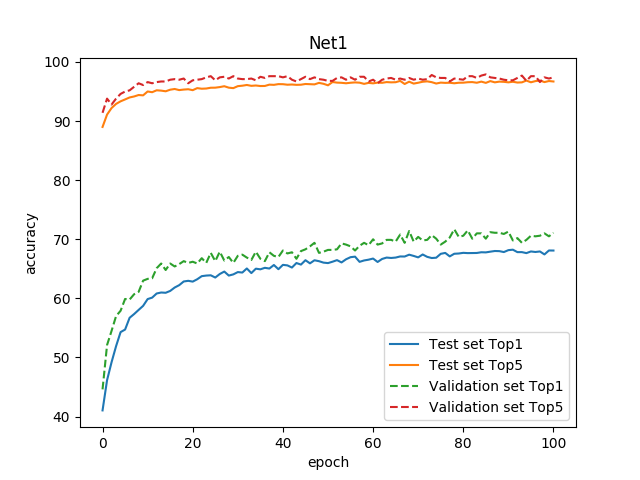
\includegraphics[width=6cm]{selfnet.png} }}
    \qquad
    \subfloat[Self-built Net Diagram]{{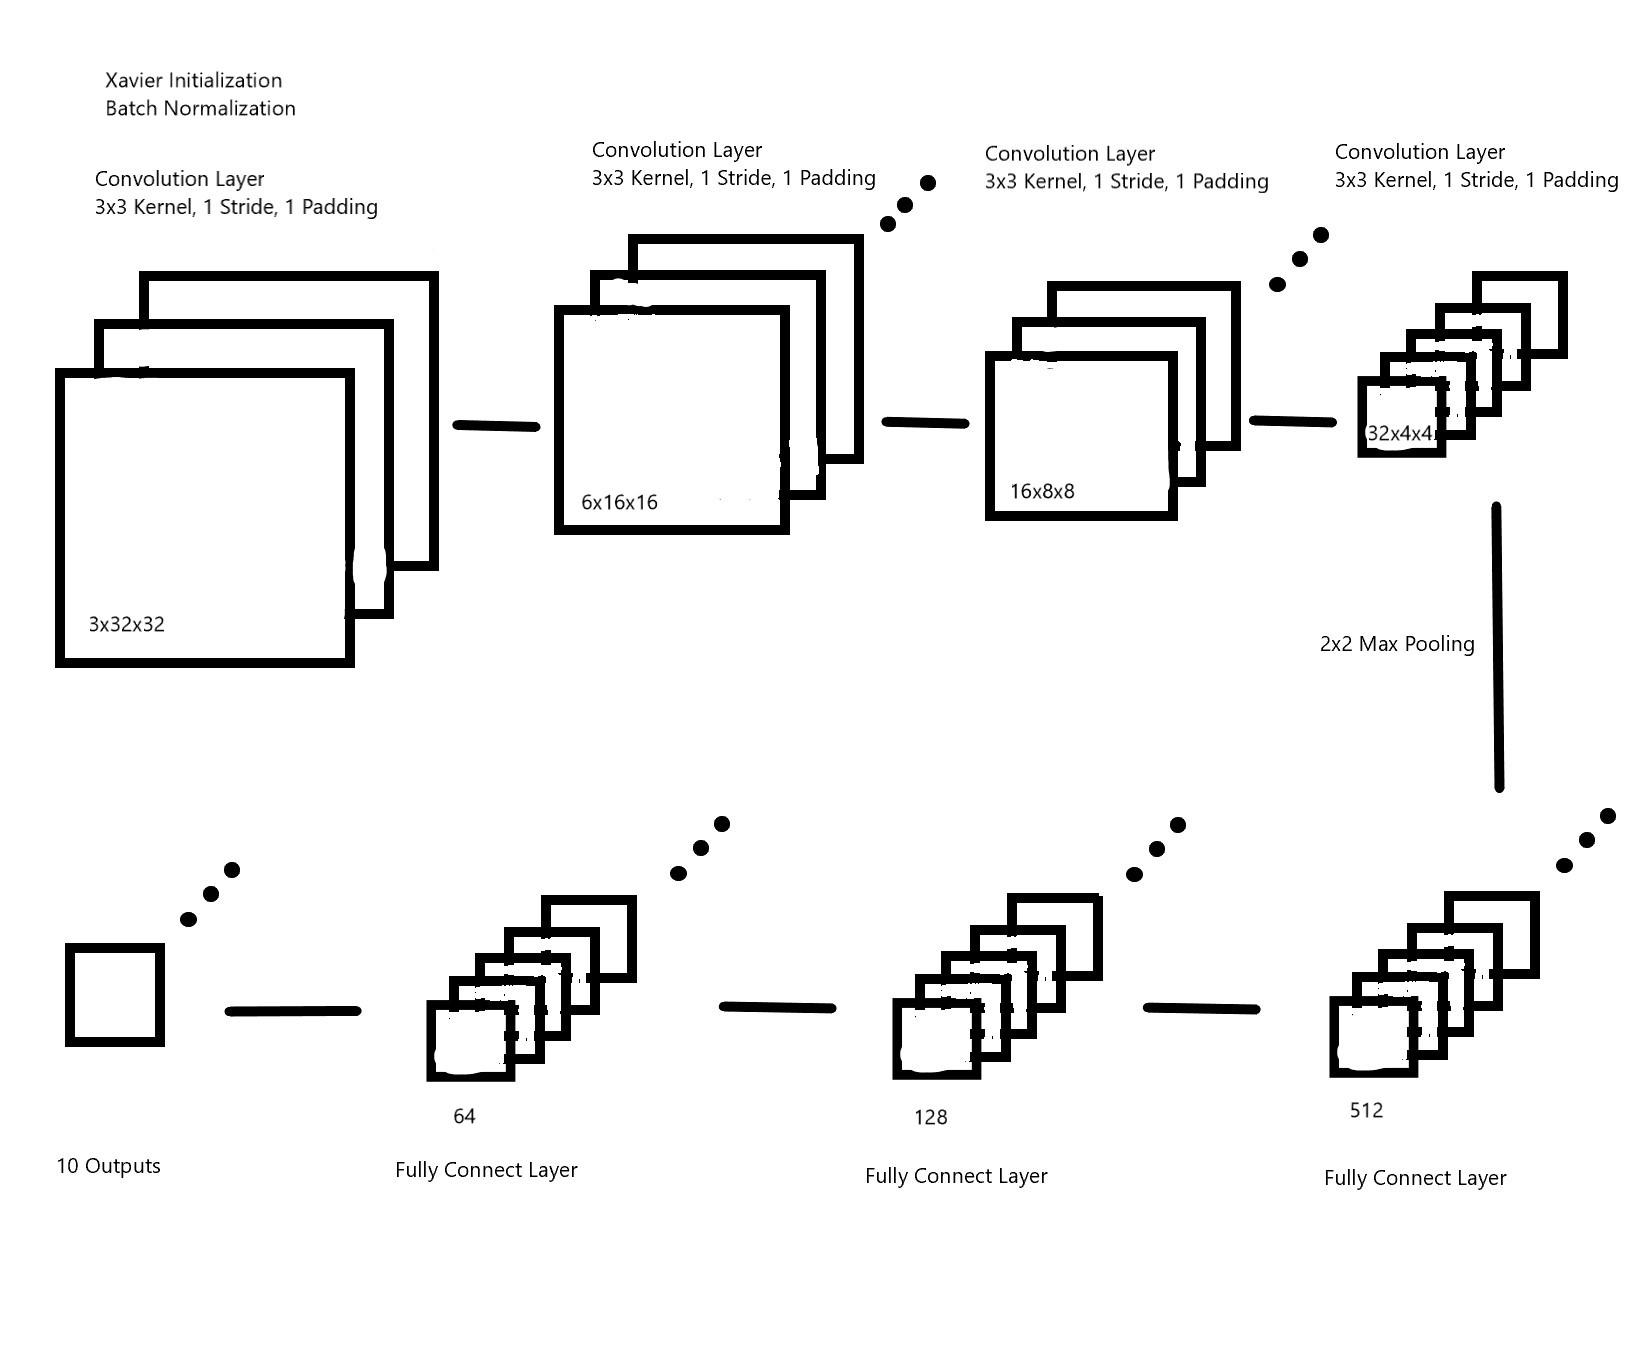
\includegraphics[width=6cm]{selfdiag.jpg} }}
    \caption{Self-built Model}
    \label{fig:self}
\end{figure}

 \subsection{GoogLeNet Model }
We used part of GoogLeNet to train our model. GoogLeNet use Inception architecture in their models. In inception model, they apply different filters on a single feature map and group them into one clusters of output. These clusters input of the next layer. According to \cite{Googlenet}, each unit from earlier layer describe some features of the input image and all passed to the next layer. Different feature maps are concatenated together into a single region and can be covered by a 1x1 convolution filter. Then several inception models are stacked on top of each other to form deep networks. Due memory efficience reason, they also proposed that it is beneficial to start using Inception modules at higher layers while keeping the lower layers in traditional convolutional fashion. In our work, we only took part of the whole GoogLeNet, first due to computation limitation and second the image size for Cifar is 32x32 compare to their 224x224 size. I also shrinked the size of convolution kernel at lower layer to take some more local features.
 \begin{figure}[h]
    \centering
    \subfloat[Accuracy vs. Epoch]{{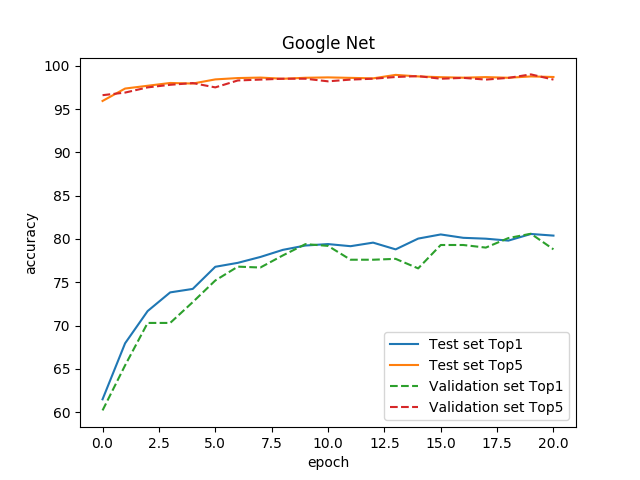
\includegraphics[width=6cm]{goolenet.png} }}
    \qquad
    \subfloat[GooLeNet Diagram]{{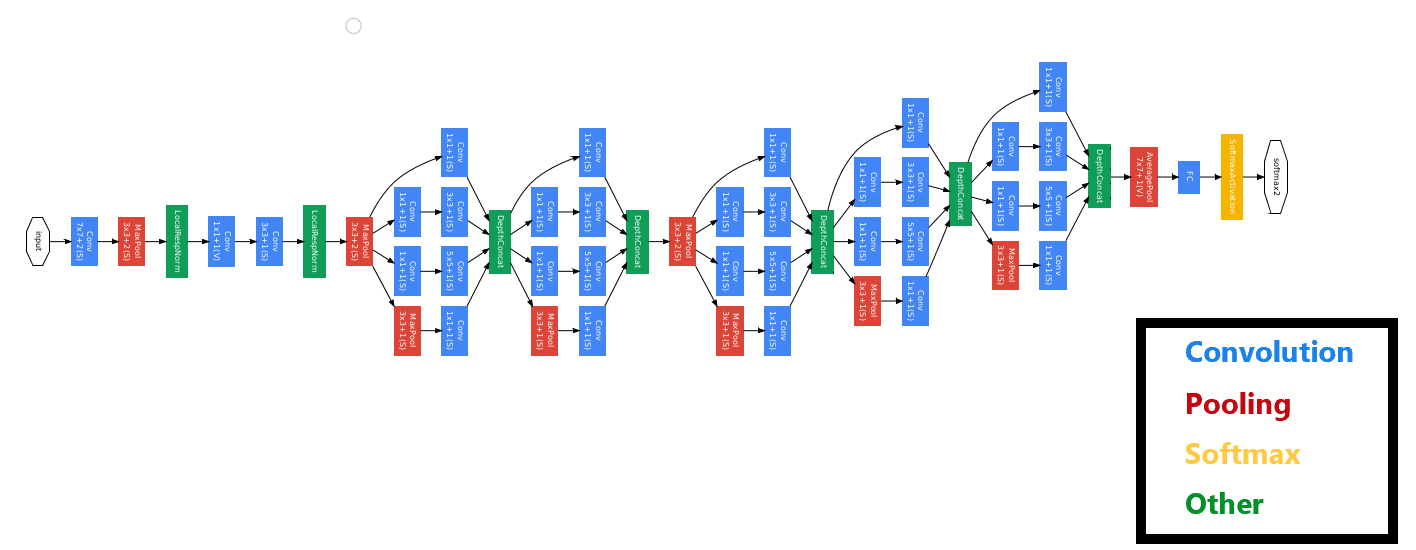
\includegraphics[width=6cm]{goodiag.png} }}
    \caption{GooLeNet Model}
    \label{fig:goog}
\end{figure}

\subsection{Discussion}
We first tried different different parameters for self-build network. First, we tried to change kernel
size to 5,5,3 for three layers. The top5 accuracy drops from $97\%$ to $95\%$. As AlexNet originally 
suggested, we tried 11x11 kernel. However, the accuracy alow drops. We suspects that in this dataset
local features are more prefered. \

Then, we replaced stochastic gradient descent with Adam. The accuracy raised from $94.1\%$ to $97.4\%$.
It also takes less epoches to converge. As suggested in \cite{adam}, the step-size is approximately bounded
by the step-size hyper-parameter and parameters update are invariant to re-scaling of gradient. Therefore, 
it can both speed up the learning process especially when it is about to converge and increase accuracy. \

We also tried Leak ReLU activation function and difference size of maxpooling. However, the difference in accuracy
and training speed is not noticeable. With leak ReLU, accuracy drop from $97\%$ to $96.2\%$ which is 
surprising since theoratically, leak ReLU should have better performance than regular ReLU.  

Generally, by comparing AlexNet, GoogLeNet and our self-built net, it is clear that GoogLeNet performs best, and AlexNet performs better than our self-built architecture. The difference between an AlexNet and our self-built architecture is that self-built net has three convolutional layer and three fully-connected layer, while AlexNet has five convolutional layer and three fully-connected layer. Their difference of two convolutional layers has result in different accuracies vs epochs, with AlexNet outperforms self-built net by 1.1\%. This simple comparison shows that given sufficient training data, a more complex function can be learned and enables the networks to more easily discriminate between different classes. The advantage of multiple layers is that they can learn features at various levels of abstraction, and are much better at generalization. This is also why in the space of 4 years, deep CNN develops from AlexNet to Residual nets (1000 layers).

From the accuracy plot for both AlexNet and GoogLeNet, we can see that GoogLeNet has a better performance compare to AlexNet. GoogLeNet is much deeper than Alexnet and takes advantage of Inception models which allows a significate amount of units in each layer. Increasing feature map can help the model to perform better and using inception model both local and global features can be captured through difference convolution kernel. Based on \cite{Googlenet}, the 1�1 convolutions are used to compute reductions before the expensive 3�3 and 5�5 convolutions. 
In terms of computation speed, the training time for GoogLeNet is doubled compare to AlexNet despite it is almost four times deeper than AlexNet. This leads to the another advantage of Inception architecture. GoogLeNet consists of several small parallel convolutions which can dramatically reduce the size of learnable parameter. Original GoogLeNet consisted of a 22 layer deep CNN but only as 4 million parameters, compare to AlexNet which has 60 million parameters. 
However, the model of GoogLeNet is not very intuitive compare to AlexNet. It is also harder to tune the parameters such as kernel size, stride, and convolution layer. It also takes GoogLeNet longer to converge.

% \section{Transfer Learning}
\IfFileExists{contrib}{\include{contrib}}{.}

\section{Conclusion}
Generally speaking, applying different tricks to neural networks does not affect much on the training results, say accuracy and loss. However, what needs to be taken into consideration is the trick parameter choices and acceleration effect tricks can have on training process. For example, weight initialization needs to be chosen randomly so that sigmoid is primarily activated in linear region.   
 
Moreover, the number of hidden nodes can have different effects on the training results. If the number of hidden nodes are too large or too small, the accuracy will drop and when the number of hidden nodes are too large, the process will be long.
 
Increase hidden layers does not affect the results of the neural network. With that being said, further experiment with more numbers of hidden layers ought to be conducted. 

\IfFileExists{contrib}{\input{contrib}}{.}

\section{Contributions}
\subsection{Siwei Guo}
1. Implement the algorithm Classification, Tricks and Topology\\
2. Explore extra credit

\subsection{Jingyi Yang}
1. Perform experiments on Classification, Tricks and Topology \\
2. Write report for all experiments.

\subsection{xxx}

\subsection{xxx}

\section{Code Reference}
Pytorch tutorial: \url{http://pytorch.org/tutorials/beginner/blitz/cifar10_tutorial.html}\

ImageNet pytorch tutorial: \url{https://github.com/pytorch/examples/blob/master/imagenet/main.py}\

GoogLeNet: \url{https://github.com/kuangliu/pytorch-cifar/blob/master/models/googlenet.py}\

%\section{Reference}
\begin{thebibliography}{9}

\bibitem{Chris Bishop} Chris Bishop, Neural Networks for Pattern Recognition.
 \emph{Oxford University Press}, 1995.
 
\bibitem{Geo}Geoffrey E Hinton, Nitish Srivastava, Alex Krizhevsky, Ilya Sutskever, and Ruslan R Salakhutdinov
 \emph{Improving neural networks by preventing co-adaptation of feature detectors}

\bibitem{google}Christian S., Wei L., Yangqing J., Pierre S., Scott R., Dragomir A., Dumitru E.,
Vincent V., Andrew R., Going Deeper with Convolutions
\emph{CVPR 2015}

\bibitem{adam}Diederik P. Kingma, Jimmy Ba., Adam: A Method for Stochastic Optimization
 \emph{3rd International Conference for Learning Representations}, 2014

\end{thebibliography}

\end{document}
